\newpage
\begin{appendices}

\chapter{Bird Daemon vs. other solutions analysis from IXNs perspective}
\label{app:ch:blinks}

On large-scale routing deployments, for example an Internet eXchange Point (IXP), the most well-known OSS solution is Quagga. However, there are other alternatives as powerful as Quagga and even less resource eater. Although Bird Daemon is a less known technology, it has presence in most of the key exchange points and its capabilities matches Quagga's and even overcomes it thanks to some key features along with an almost negligible resource consumption in comparison to other solutions.

After looking for good references and projects about IXPs implementing and analysing Bird Daemon and asking its community, I have triaged some relevant presentations showing Bird's potential and its increasing interest over the years, along with the complexity of the solutions implemented:

\begin{itemize}
    \item Amsterdam Internet eXchange (AMSIX): 2010 presentation analysing the use of different routing solutions and resource consumption data. \href{http://ripe60.ripe.net/presentations/Jasinska-_Ab_Using_Route_Servers.pdf}{\nolinkurl{http://ripe60.ripe.net/presentations/Jasinska-\_Ab\_Using\_Route\_Servers.pdf}}
    
    \item AMSIX (II): 2012 presentation analysing different routing implementations in a specific testbed. \href{https://ams-ix.net/downloads/ams-ix-route-server-implementations-performance.pdf}{https://ams-ix.net/downloads/ams-ix-route-server-implementations-performance.pdf}

    \item CZ.NIC (Bird core developers): 2013 presentation in NANOG57 conference about the latest version of Bird Daemon, key IXP using it and features added since the previous NANOG conference the developers attended to. \href{https://www.nanog.org/meetings/nanog57/presentations/Wednesday/wed.general.Filip.BIRD.16.pdf}{\nolinkurl{https://www.nanog.org/meetings/nanog57/presentations/Wednesday/wed.general.Filip.BIRD.16.pdf}}

    \item DE-CIX: 2016 presentation in RIPE73 conference about scaling Bird servers to load-balance queries. \url{https://ripe73.ripe.net/presentations/115-e-bru-20161026-RIPE73-scaling-bird-routeservers-final.pdf}
    
    \item DE-CIX: 2017 presentation in Euro-IX conference showing a framework developed in order to generate stress tests in large-scale BGP sessions to automate these tests with minimum impact in their infrastructure. \url{https://euro-ix.net/m/filer_public/81/dd/81dda868-dd3b-46be-8ee2-9881d112af5a/de-cix_route_server_testframework_euro-ix_30.pdf}
\end{itemize}


\chapter{Kanban Project Management using Taiga.io Service}
\label{app:sec:kanban}
As part of the initial investigation, I did some research on Open Source Project Management tools that could help me monitoring my progress as well as adding some value to the final project.
Because of this project's scope and time-frame, the size of the team (me) and the number of Stakeholders (Víctor), the only Agile \textit{approach} that I could use was Kanban\footnote{\href{http://www.scrumhub.com/kanban-fundamentals/}{Kanban} approach summarised: project with a continuous prioritised backlog, one task per team resource, the project must be releasable after closing any task, reduce to the minimum the number of required ceremonies and tasks go from \textit{ToDo} (left) to \textit{Done} (right).}. The following sections present the tests and initial usage of Taiga Kanban service.

\begin{landscape}
\section{EPICS View}
\begin{figure}[h!]
\centering
    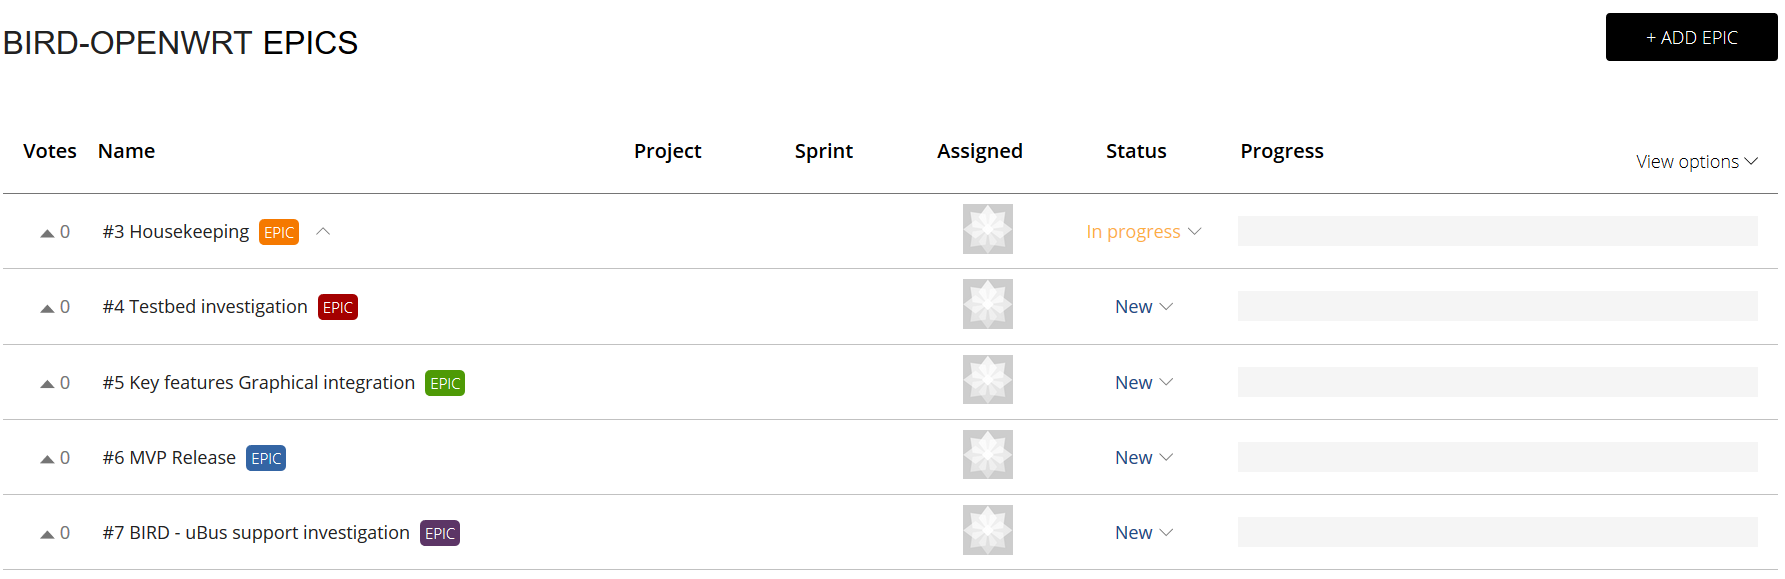
\includegraphics[width=\hsize]{images/kanban/epics}
    \caption{Project EPICs overview}
    \label{fig:kepic}
\end{figure}

This view presents the information about the big tasks represented in project's schedule, who is working on each one, other useful information and how far is the task from being delivered.
\newpage

\subsection{EPIC Detail View}
\begin{figure}[h!]
\centering
    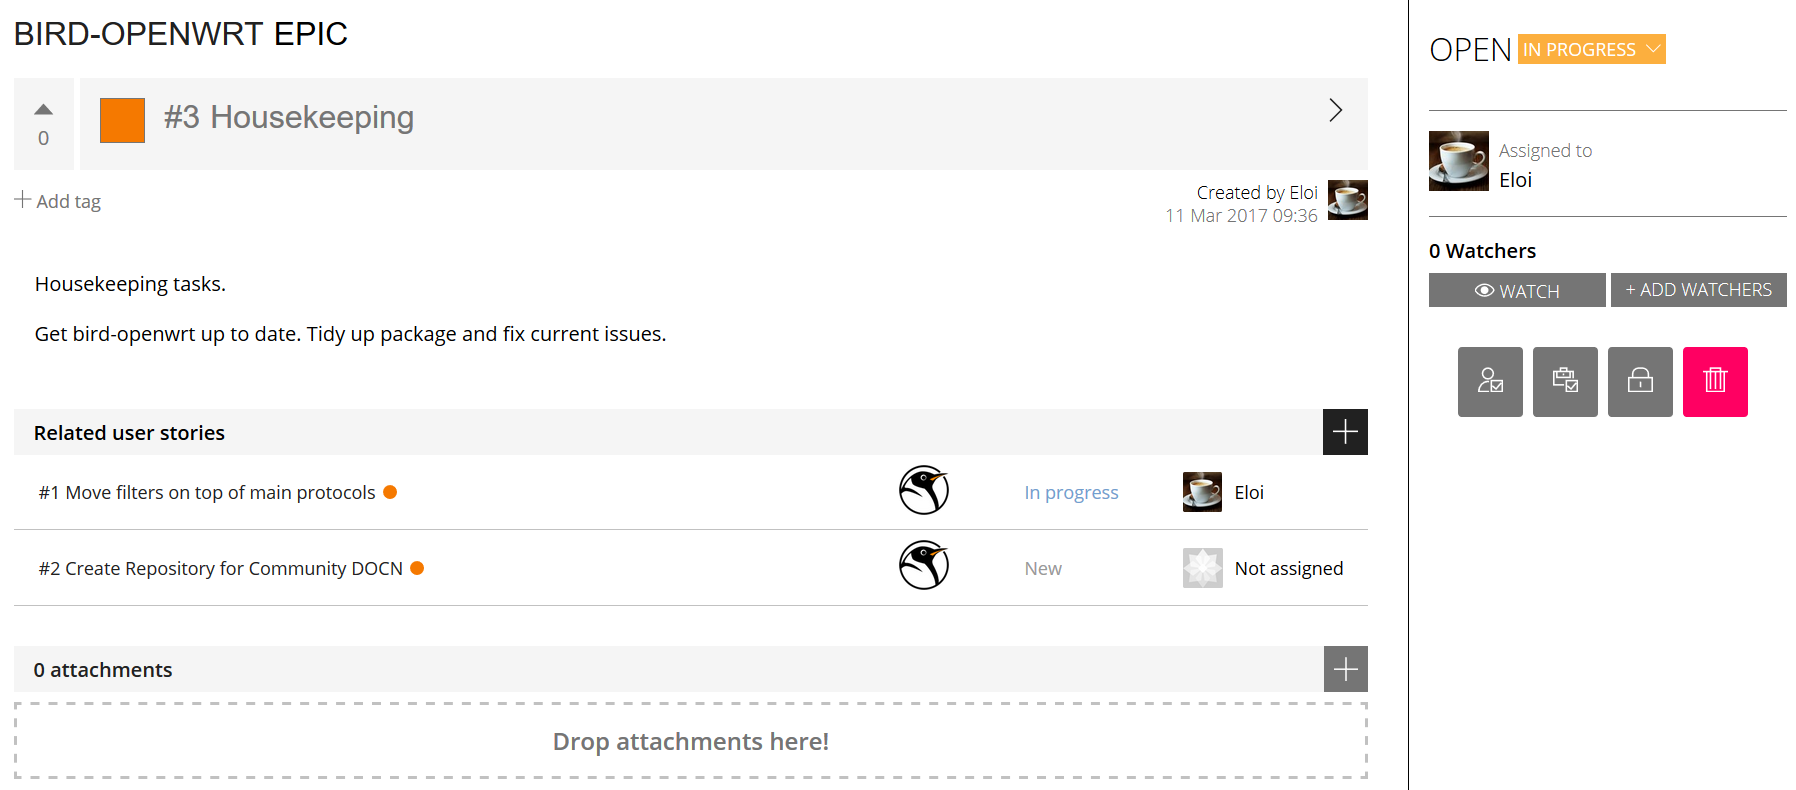
\includegraphics[width=0.85\hsize]{images/kanban/epic-details}
    \caption{Housekeeping EPIC detailed view}
    \label{fig:kepicd}
\end{figure}
This view presents the detailed information of a specific Epic. It presents the first EPIC \textit{Housekeeping} which is In Progress, assigned to \textit{Eloi} and two tasks, one already in progress and another waiting for resources.
\newpage

\section{Timeline View}
\begin{figure}[h!]
\centering
    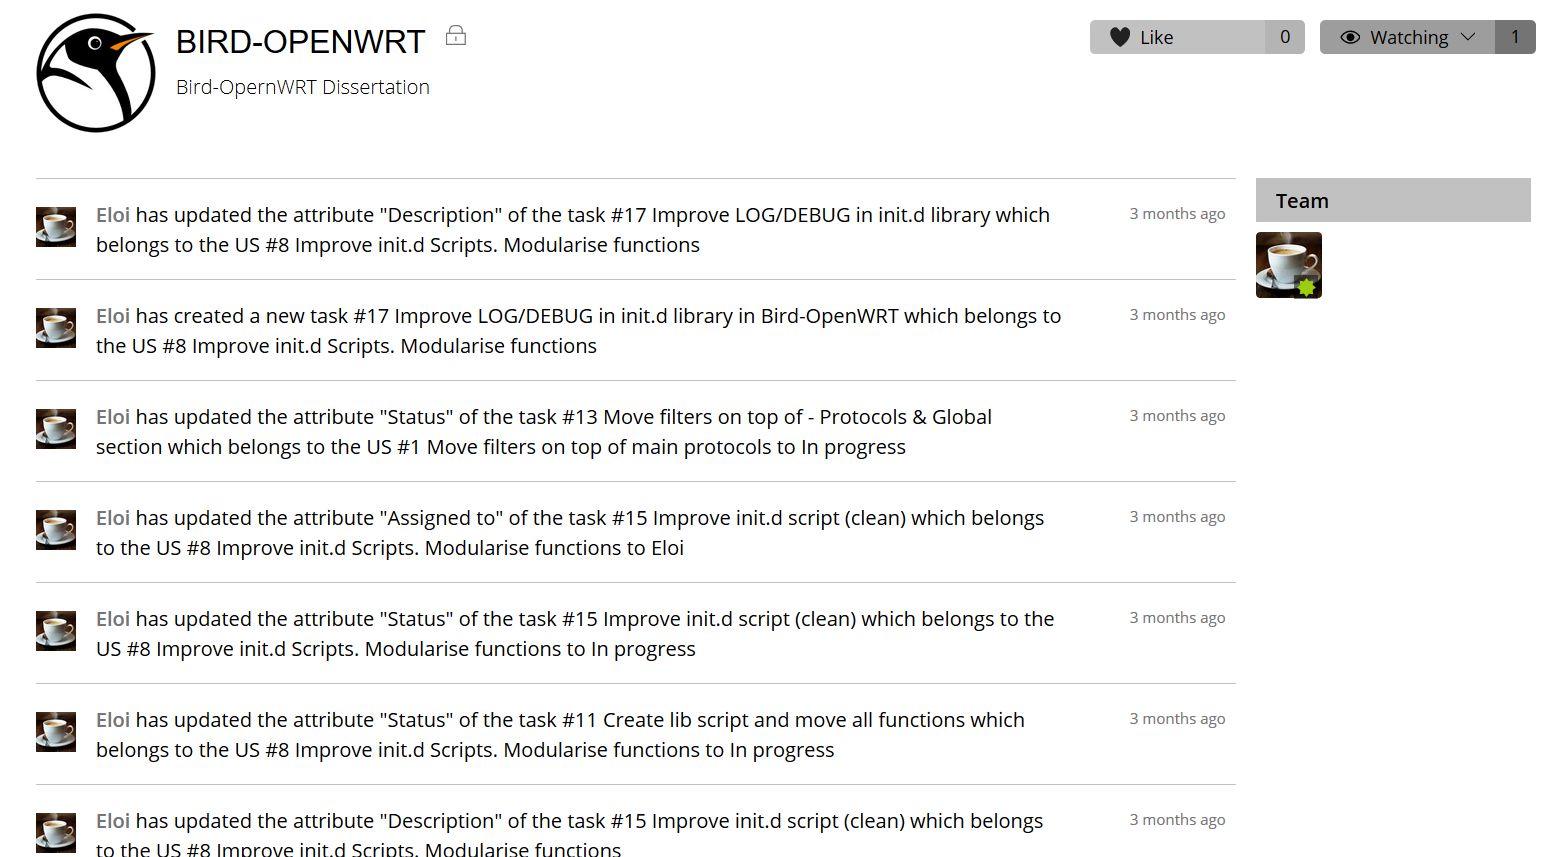
\includegraphics[width=0.7\hsize]{images/kanban/timeline}
    \caption{Project timeline status information}
    \label{fig:ktimeline}
\end{figure}
The Timeline View presents Project's log information. Any action applied to any of the tasks, stories or epics will be logged and shown chronologically in this page.
\newpage

\section{Kanban Board View}
\begin{figure}[ht!]
\centering
    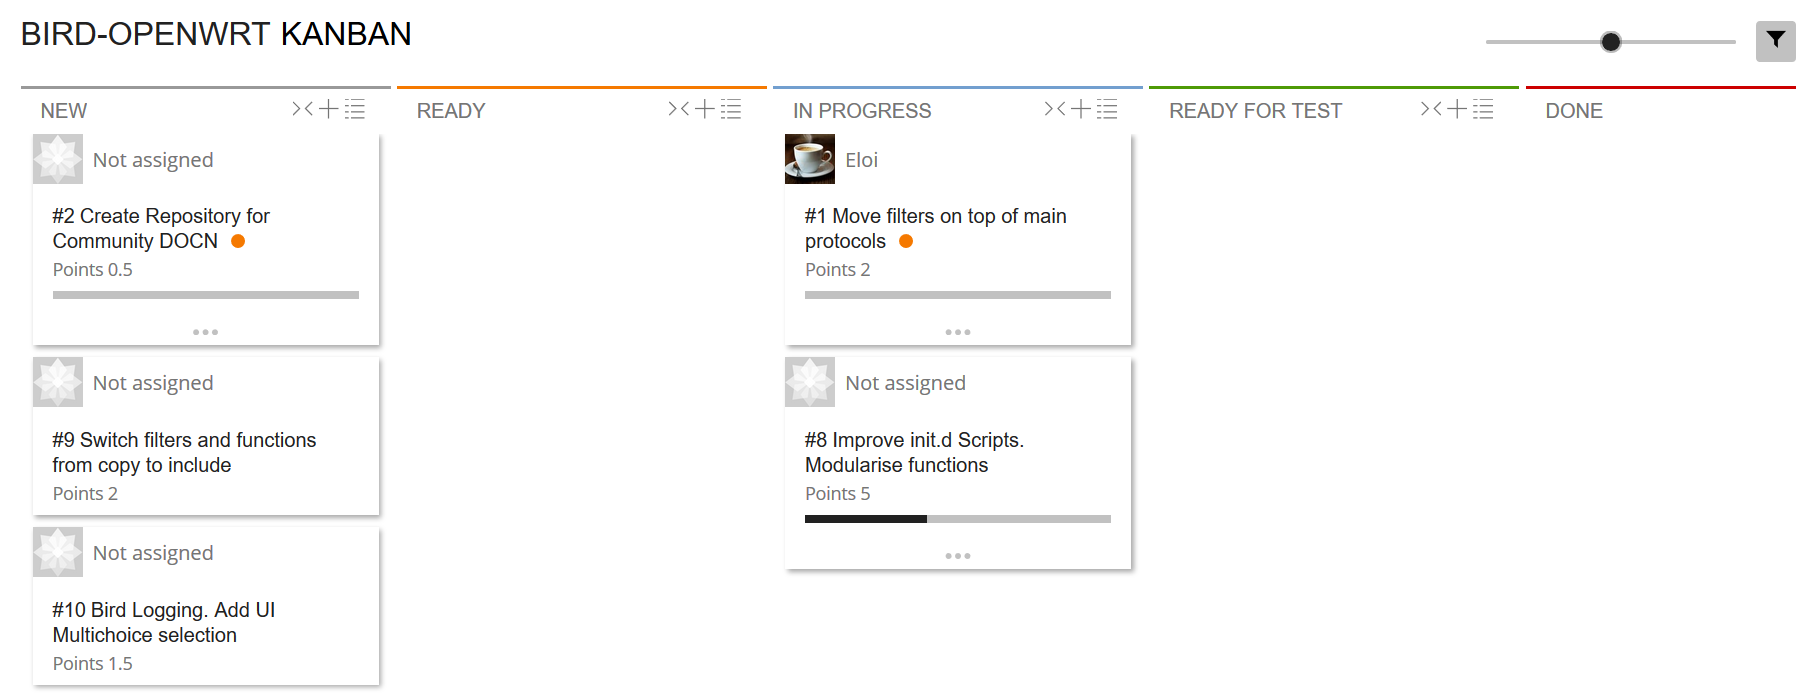
\includegraphics[width=0.85\hsize]{images/kanban/kanban}
    \caption{Kanban User Stories board view}
    \label{fig:kboard}
\end{figure}
The Kanban Board shows the state of the User Stories being addressed, in which state and how far they are from being completed.
\newpage

\subsection{Cycle/Sprint View}
\begin{figure}[ht!]
\centering
    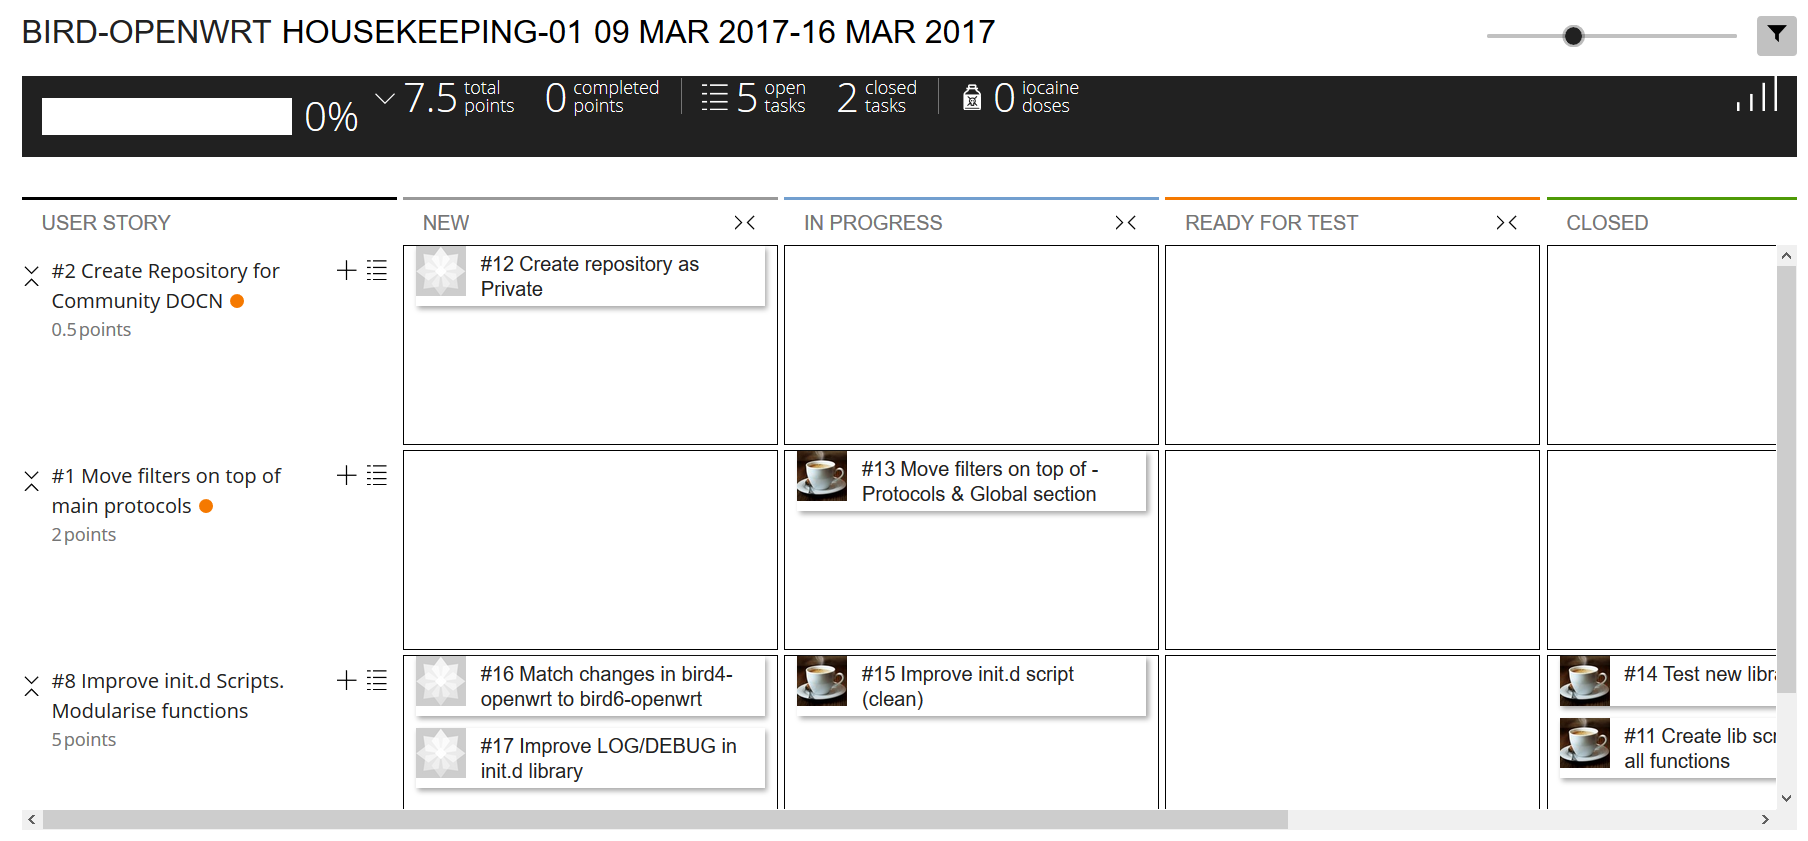
\includegraphics[width=0.85\hsize]{images/kanban/cycle}
    \caption{Kanban current cycle/sprint tasks board view}
    \label{fig:kcycle}
\end{figure}
The Cycle/Sprint View presents the user stories being addressed in priority order (in the left) and all the involved Tasks required to complete each of these user stories, to who they are assigned and their state. This is a detailed view of the Kanban Board View.

\end{landscape}

\chapter{Extra LUCI Example Pages}
\label{app:ch:extrap}

\section{Privoxy LUCI2 Status Page}
\begin{figure}[H]
    \centering
    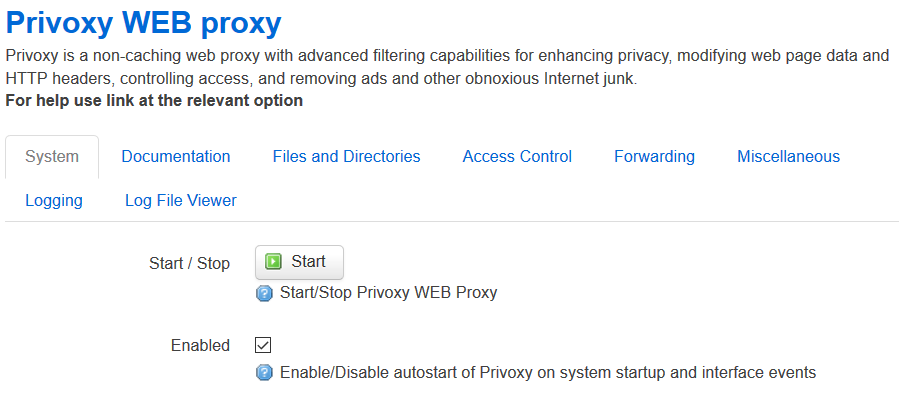
\includegraphics[width=0.95\textwidth]{images/luciextra/disabled}
    \caption{Privoxy disabled service.}
    \label{fig:privdis}
\end{figure}

\begin{figure}[H]
    \centering
    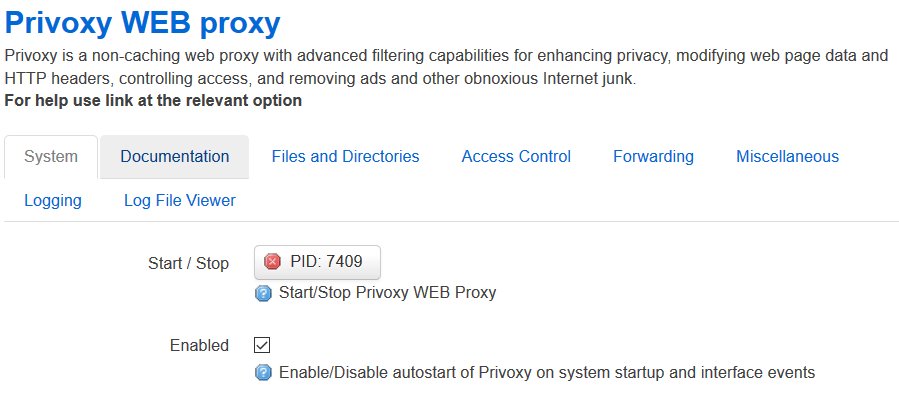
\includegraphics[width=0.95\textwidth]{images/luciextra/enabled}
    \caption{Privoxy enabled service.}
    \label{fig:priven}
\end{figure}

\chapter{Bird Daemon's Configuration using v0.3 Package - UOC's VM in Guifi.net}
\label{app:ch:bdcuoc}

\section{UCI Configuration}
\begin{lstlisting}[language=bash,caption={UCI Configuration}]
config bird 'bird'
        option use_UCI_config '1'
        option UCI_config_file '/tmp/bird4.conf'
        option UCI_config_File '/tmp/bird4.conf'

config global 'global'
        option log_file '/tmp/bird4.log'
        option router_id '10.139.173.161'
        option log 'all'

config table
        option name 'aux'

config kernel 'kernel1'
        option import 'all'
        option export 'all'
        option scan_time '10'
        option learn '1'
        option disabled '0'

config device 'device1'
        option scan_time '10'
        option disabled '0'

config bgp_template 'BGP_COMMON'
        option receive_limit_action 'warn'
        option local_as '92099'
        option igp_table 'bgpTable'
        option export_limit_action 'warn'
        option import_limit_action 'warn'
        option next_hop_self '0'
        option next_hop_keep '0'
        option rr_client '0'

config table
        option name 'bgpTable'

config bgp 'BGPImportALL'
        option receive_limit_action 'warn'
        option template 'BGP_COMMON'
        option neighbor_as '59361'
        option neighbor_address '172.25.35.25'
        option export_limit_action 'warn'
        option import_limit_action 'warn'
        option import_limit '3000'
        option import 'filter ebgp_in'
        option export 'filter ebgp_out'
        option next_hop_self '0'

config kernel 'Kernel_BGP'
        option disabled '0'
        option table 'bgpTable'
        option kernel_table '251'
        option scan_time '10'
        option learn '1'
        option import 'all'
        option export 'all'

config pipe 'pipe1'
        option disabled '0'
        option peer_table 'bgpTable'
        option table 'aux'
        option import 'all'
        option export 'all'
        option mode 'transparent'

config direct 'direct1'
        option disabled '0'
        option interface '"br-lan","br-wan", "br-mgmt"'

config static 'static1'
        option disabled '0'
        option table 'aux'
\end{lstlisting}

\section{Bird Configuration}
\begin{lstlisting}[language=bash,caption={Bird4.conf Configuration}]
#Bird4 configuration using UCI:

log "/tmp/bird4.log" all;

#Router ID
router id 10.139.173.161;

#Secondary tables
table aux;
table bgpTable;

#Functions Section:
include "/etc/bird4/functions/function-20170507-1038";
#End of Functions --

#Filters Section:
include "/etc/bird4/filters/filter-20170507-0951";
#End of Filters --

#kernel1 configuration:
protocol kernel kernel1 {
#   disabled;
    learn;
    persist;
    scan time 10;
    import all;
    export all;
}

#Kernel_BGP configuration:
protocol kernel Kernel_BGP {
#   disabled;
    table bgpTable;
    kernel table 251;
    learn;
    persist;
    scan time 10;
    import all;
    export all;
}

#static1 configration:
protocol static {
    table aux;
}

#device1 configuration:
protocol device {
#   disabled;
    scan time 10;
}

#direct1 configuration:
protocol direct {
#   disabled;
    interface "br-lan","br-wan", "br-mgmt";
}

#pipe1 configuration:
protocol pipe pipe1 {
#   disabled;
    table aux;
    peer table bgpTable;
    mode transparent;
    import all;
    export all;
}

#BGP_COMMON template:
template bgp BGP_COMMON {
    local as 92099;
#    next hop self;
#    next hop keep;
    igp table bgpTable;
#    rr client;
}

#BGPImportALL configuration:
protocol bgp BGPImportALL from BGP_COMMON {
    import filter ebgp_in;
    export filter ebgp_out;
#    rr client;
    import limit 3000 action warn;
    neighbor 172.25.35.25 as 59361;
}

========================================
BGP Filters and Functions:
root@LEDE-eloi:~# cat /etc/bird4/filters/filter-20170507-0951
filter ebgp_in {

        krt_prefsrc = 10.139.173.161;

        if match_guifi_prefix() then accept;
        reject;
}

filter ebgp_out {

        if match_guifi_prefix() then accept;
        reject;
        

root@LEDE-eloi:~# cat /etc/bird4/functions/function-20170507-1038
function match_guifi_prefix()
{
        return net ~ [ 10.0.0.0/8{9,32} ];
}
\end{lstlisting}

%%%%%%%%%%%%%%%%%%%%%%%%%%%%%%%%%%%%%%%%%%%%%%%%%%%%%%%%%%%%%%%%%%%%%%%%%%%%%%%%%%

\chapter{Final Package's Tests configuration files}
\label{app:ch:full}
Configuration files used in the tests explained in the Section \ref{sub:fulltest}.

\section{Mesh eXchange Node 1 (MXN1)}
\begin{lstlisting}[language=bash, caption={Network}]
config interface 'loopback'
        option ifname 'lo'
        option proto 'static'
        option ipaddr '127.0.0.1'
        option netmask '255.0.0.0'

config globals 'globals'
        option ula_prefix 'fd96:db1d:bd49::/48'

config interface 'mgmt'
        option type 'bridge'
        option ifname 'eth0'
        option proto 'static'
        option ipaddr '192.168.5.2'
        option netmask '255.255.255.0'

config interface 'wan'
        option type 'bridge'
        option ifname 'eth1'
        option proto 'static'
        option ipaddr '172.25.35.26'
        option netmask '255.255.255.252'

config interface 'lan'
        option type 'bridge'
        option ifname 'eth2'
        option proto 'static'
        option ip6assign '64'

config interface 'mesh'
        option ifname 'eth3'
        option _orig_ifname 'eth3'
        option _orig_bridge 'false'
        option proto 'static'
        option ipaddr '10.90.236.97'
        option netmask '255.255.255.224'
\end{lstlisting}
\begin{lstlisting}[language=bash, caption={BMX6}]
config bmx6 'general'
        option tun4Address '10.90.236.97/27'
        option tun6Address '2012:0:0:a7fa:0:0:0:1/64'

config plugin 'bmx6_config_plugin'
        option plugin 'bmx6_config.so'

config plugin 'bmx6_json_plugin'
        option plugin 'bmx6_json.so'

config plugin 'bmx6_sms_plugin'
        option plugin 'bmx6_sms.so'

config plugin 'bmx6_table_plugin'
        option plugin 'bmx6_table.so'

config syncSms
        option syncSms 'chat'

config dev 'mesh_1'
        option dev 'eth3'
        option linklayer '1'
        option rateMin '56000000'
        option rateMax '56000000'

config tunDev 'tmain'
        option tunDev 'tmain'
        option tun4Address '10.90.236.97/27'
        option tun6Address '2012:0:0:a7fa:0:0:0:1/64'

config tunOut 'mesh_cloud'
        option network '10.0.0.0/8'
        option tunOut 'cloud'
        option minPrefixLen '24'

config tunOut 'mesh_cloud6'
        option network '::/0'
        option tunOut 'cloud6'
        option minPrefixLen '48'

config tunIn 'mesh_offer'
        option tunIn 'offer'
        option network '10.0.0.0/8'

config redistTable 'bgp'
        option redistTable 'bgp'
        option table '251'
        option network '10.0.0.0/8'
        option aggregatePrefixLen '24'
        option minPrefixLen '8'
        option maxPrefixLen '29'
        option all '1'

config tunOut
        option tunOut 'community'
        option network '10.0.0.0/8'
        option maxPrefixLen '8'
\end{lstlisting}
\begin{lstlisting}[language=bash, caption={Bird Filters}]
filter ebgp_in {

        krt_prefsrc = 10.90.236.97;

        if match_guifi_prefix() then accept;
        else reject;
}

filter ebgp_out {

        if match_guifi_prefix() then accept;
        else reject;
}

filter ibgp_in {
        if match_guifi_prefix() then accept;
        else reject;
}

filter ibgp_out {
        if match_guifi_prefix() then accept;
        else reject;
}

filter accept_from_peer_BCNRamblaPobleNou {
        if proto="BCNRamblaPobleNou" then accept;
        else reject;
}

filter reject_no_zone2_prefix {
        if match_zone2_prefix() then accept;
        else reject;
}

filter accept_zone1_prefix {
        if match_zone1_prefix() then accept;
        else reject;
}

filter reject_from_peer_UOCBGPMesh {
        if proto="UOCBGPMesh" then reject;
        else accept;
\end{lstlisting}
\begin{lstlisting}[language=bash, caption={Bird Functions}]
function match_guifi_prefix()
{
        return net ~ [ 10.0.0.0/8{9,32} ];
}

function match_zone1_prefix() {
        return net ~ [
                10.1.24.0/21{24,28},
                10.139.6.0/23{24,28},
                10.139.16.0/20{24,28},
                10.139.36.0/22{24,28},
                10.139.173.0/24{24,28},
                10.90.224.0/20{24,28},
                10.228.192.0/20{24,28},
                10.38.140.0/22{24,28}
        ];

}

function match_zone2_prefix() {
        return net ~ [ 10.90.236.0/23{24,28} ];
\end{lstlisting}
\begin{lstlisting}[language=bash, caption={Bird UCI}]
config bird 'bird'
        option use_UCI_config '1'
        option UCI_config_file '/tmp/bird4.conf'
        option UCI_config_File '/tmp/bird4.conf'

config global 'global'
        option log_file '/tmp/bird4.log'
        option router_id '10.90.236.97'
        option log 'all'

config kernel 'kernel1'
        option import 'all'
        option scan_time '10'
        option learn '1'
        option disabled '0'
        option kernel_table '251'
        option table 'bgpTable'
        option export 'filter accept_zone1_prefix'

config device 'device1'
        option scan_time '10'
        option disabled '0'

config direct 'direct1'
        option disabled '0'
        option interface '"br-lan", "eth3"'

config bgp_template 'bgpCommon'
        option export_trigger '0'
        option receive_trigger '0'
        option local_as '92099'
        option import 'all'
        option export 'all'
        option import_trigger '0'

config bgp 'BCNRamblaPobleNou'
        option export_trigger '0'
        option receive_trigger '0'
        option disabled '0'
        option template 'bgpCommon'
        option neighbor_address '172.25.35.25'
        option neighbor_as '59361'
        option import_trigger '0'
        option import 'filter ebgp_in'
        option export 'filter ebgp_out'
        option table 'bgpTable'

config bgp 'UOCBGPMesh'
        option import_trigger '0'
        option export_trigger '0'
        option receive_trigger '0'
        option template 'bgpCommon'
        option neighbor_address '10.90.236.1'
        option neighbor_as '92099'
        option disabled '0'
        option table 'bgpTable'
        option import 'filter ibgp_in'
        option export 'filter ibgp_out'
        option igp_table 'master'
        option next_hop_self '1'

config table
        option name 'bgpTable'

config table
        option name 'master'

config kernel 'kernel2'
        option disabled '0'
        option import 'all'
        option export 'all'
        option learn '1'
        option scan_time '10'

config pipe 'pipe1'
        option disabled '0'
        option mode 'transparent'
        option table 'master'
        option peer_table 'bgpTable'
        option import 'filter accept_from_peer_BCNRamblaPobleNou'
        option export 'filter reject_no_zone2_prefix'
\end{lstlisting}
\begin{lstlisting}[language=bash, caption={Birdc RAW Configuration}]
#Bird4 configuration using UCI:

log "/tmp/bird4.log" all;

#Router ID
router id 10.90.236.97;

#Secondary tables
table bgpTable;
table master;

#Functions Section:
include "/etc/bird4/functions/function-20170507-1038";
#End of Functions --

#Filters Section:
include "/etc/bird4/filters/filter-20170507-0951";
#End of Filters --

#kernel1 configuration:
protocol kernel kernel1 {
#   disabled;
    table bgpTable;
    kernel table 251;
    learn;
    persist;
    scan time 10;
    import all;
    export filter accept_zone1_prefix;
}

#kernel2 configuration:
protocol kernel kernel2 {
#   disabled;
    learn;
    persist;
    scan time 10;
    import all;
    export all;
}

#device1 configuration:
protocol device {
#   disabled;
    scan time 10;
}

#direct1 configuration:
protocol direct {
#   disabled;
    interface "br-lan", "eth3";
}

#pipe1 configuration:
protocol pipe pipe1 {
#   disabled;
    table master;
    peer table bgpTable;
    mode transparent;
    import filter accept_from_peer_BCNRamblaPobleNou;
    export filter reject_no_zone2_prefix;
}

#bgpCommon template:
template bgp bgpCommon {
    local as 92099;
    import all;
    export all;
#    rr client;
}

#BCNRamblaPobleNou configuration:
protocol bgp BCNRamblaPobleNou from bgpCommon {
#   disabled;
    table bgpTable;
    import filter ebgp_in;
    export filter ebgp_out;
#    rr client;
    neighbor 172.25.35.25 as 59361;
}

#UOCBGPMesh configuration:
protocol bgp UOCBGPMesh from bgpCommon {
#   disabled;
    table bgpTable;
    import filter ibgp_in;
    export filter ibgp_out;
    igp table master;
    next hop self;
#    rr client;
    neighbor 10.90.236.1 as 92099;
}
\end{lstlisting}
\begin{lstlisting}[language=bash, caption={Birdc4 show protocols all}]
BIRD 1.6.3 ready.
name     proto    table    state  since       info
kernel1  Kernel   bgpTable up     13:41:23
  Preference:     10
  Input filter:   ACCEPT
  Output filter:  accept_zone1_prefix
  Routes:         0 imported, 169 exported, 0 preferred
  Route change stats:     received   rejected   filtered    ignored   accepted
    Import updates:              0          0          0          0          0
    Import withdraws:            0          0        ---          0          0
    Export updates:          45213         20      43487        ---       1706
    Export withdraws:         6834        ---        ---        ---        427

kernel2  Kernel   master   up     13:41:23
  Preference:     10
  Input filter:   ACCEPT
  Output filter:  ACCEPT
  Routes:         97 imported, 2922 exported, 33 preferred
  Route change stats:     received   rejected   filtered    ignored   accepted
    Import updates:            490          0          0          0        490
    Import withdraws:          393          0        ---          0        393
    Export updates:          20783        279          0        ---      20504
    Export withdraws:         5461        ---        ---        ---       5371

device1  Device   master   up     13:41:23
  Preference:     240
  Input filter:   ACCEPT
  Output filter:  REJECT
  Routes:         0 imported, 0 exported, 0 preferred
  Route change stats:     received   rejected   filtered    ignored   accepted
    Import updates:              0          0          0          0          0
    Import withdraws:            0          0        ---          0          0
    Export updates:              0          0          0        ---          0
    Export withdraws:            0        ---        ---        ---          0

direct1  Direct   master   up     13:41:23
  Preference:     240
  Input filter:   ACCEPT
  Output filter:  REJECT
  Routes:         1 imported, 0 exported, 2 preferred
  Route change stats:     received   rejected   filtered    ignored   accepted
    Import updates:              1          0          0          0          1
    Import withdraws:            0          0        ---          0          0
    Export updates:              0          0          0        ---          0
    Export withdraws:            0        ---        ---        ---          0

pipe1    Pipe     master   up     13:41:23    => bgpTable
  Preference:     70
  Input filter:   accept_from_peer_BCNRamblaPobleNou
  Output filter:  reject_no_zone2_prefix
  Routes:         2922 imported, 4 exported
  Route change stats:     received   rejected   filtered    ignored   accepted
    Import updates:          46874          7      26363          0      20504
    Import withdraws:        21288          0        ---      15915       5371
    Export updates:          20996      20504        485          1          6
    Export withdraws:         5764          0        ---        391          2

BCNRamblaPobleNou BGP      bgpTable up     13:41:27    Established
  Preference:     100
  Input filter:   ebgp_in
  Output filter:  ebgp_out
  Routes:         2922 imported, 2808 exported, 3066 preferred
  Route change stats:     received   rejected   filtered    ignored   accepted
    Import updates:          20508          0          0          4      20504
    Import withdraws:         5395          0        ---         24       5371
    Export updates:          45213      23103          0        ---      22110
    Export withdraws:         6834        ---        ---        ---      14858
  BGP state:          Established
    Neighbor address: 172.25.35.25
    Neighbor AS:      59361
    Neighbor ID:      10.90.224.65
    Neighbor caps:    refresh AS4
    Session:          external AS4
    Source address:   172.25.35.26
    Hold timer:       166/180
    Keepalive timer:  17/60

UOCBGPMesh BGP      bgpTable up     13:42:52    Established
  Preference:     100
  Input filter:   ibgp_in
  Output filter:  ibgp_out
  Routes:         2837 imported, 147 exported, 2805 preferred
  Route change stats:     received   rejected   filtered    ignored   accepted
    Import updates:          23312          0          0          2      23310
    Import withdraws:        12914          0        ---          0      12914
    Export updates:          41943      19075          0        ---      22868
    Export withdraws:         6754        ---        ---        ---      13872
  BGP state:          Established
    Neighbor address: 10.90.236.1
    Neighbor AS:      92099
    Neighbor ID:      10.90.236.1
    Neighbor caps:    refresh enhanced-refresh restart-aware AS4
    Session:          internal multihop AS4
    Source address:   10.90.236.97
    Hold timer:       232/240
    Keepalive timer:  60/80
\end{lstlisting}


\section{Mesh eXchange Node 2 (MXN2)}
\begin{lstlisting}[language=bash, caption={Network}]
config interface 'loopback'
        option ifname 'lo'
        option proto 'static'
        option ipaddr '127.0.0.1'
        option netmask '255.0.0.0'

config globals 'globals'
        option ula_prefix 'fd96:db1d:bd49::/48'

config interface 'mgmt'
        option type 'bridge'
        option ifname 'eth0'
        option proto 'static'
        option ipaddr '192.168.5.5'
        option netmask '255.255.255.0'

config interface 'lan'
        option ifname 'eth2'
        option proto 'static'
        option ipaddr '84.88.58.130'
        option netmask '255.255.255.248'
        option dns '8.8.8.8'

config interface 'mesh'
        option ifname 'eth1'
        option proto 'static'
        option _orig_ifname 'eth1'
        option _orig_bridge 'false'
        option ipaddr '10.90.236.1'
        option netmask '255.255.255.224'

config interface 'upfl'
        option proto 'l2tp'
        option server '84.89.138.19'
        option username 'uoc'
        option password 'testbed'
        option ipv6 'auto'
        option defaultroute '0'

config route
        option interface 'lan'
        option target '84.89.138.19/32'
        option gateway '84.88.58.129'
\end{lstlisting}
\begin{lstlisting}[language=bash, caption={BMX6}]
config bmx6 'general'
        option tun4Address '10.90.236.1/27'
        option tun6Address '2012:0:0:a7f9:0:0:0:1/64'

config plugin 'bmx6_config_plugin'
        option plugin 'bmx6_config.so'

config plugin 'bmx6_json_plugin'
        option plugin 'bmx6_json.so'

config plugin 'bmx6_sms_plugin'
        option plugin 'bmx6_sms.so'

config plugin 'bmx6_table_plugin'
        option plugin 'bmx6_table.so'

config syncSms
        option syncSms 'chat'

config dev 'mesh_1'
        option dev 'eth1'
        option linklayer '1'
        option rateMin '56000000'
        option rateMax '56000000'

config tunDev 'tmain'
        option tunDev 'tmain'
        option tun4Address '10.90.236.1/27'
        option tun6Address '2012:0:0:a7f9:0:0:0:1/64'

config tunOut 'mesh_cloud'
        option network '10.0.0.0/8'
        option minPrefixLen '24'
        option tunOut 'cloud'

config tunOut 'mesh_cloud6'
        option tunOut 'cloud6'
        option network '::/0'
        option minPrefixLen '48'

config tunIn 'mesh_offer'
        option tunIn 'offer'
        option network '10.0.0.0/8'

config redistTable 'bgp'
        option redistTable 'bgp'
        option table '251'
        option network '10.0.0.0/8'
        option aggregatePrefixLen '24'
        option minPrefixLen '8'
        option maxPrefixLen '29'
        option all '1'

config tunOut
        option tunOut 'community'
        option network '10.0.0.0/8'
        option maxPrefixLen '8'
\end{lstlisting}
\begin{lstlisting}[language=bash, caption={Bird Functions}]
filter ebgp_in {

        krt_prefsrc = 10.90.236.1;

        if match_guifi_prefix() then accept;
        else reject;
}

filter ebgp_out {

        if match_guifi_prefix() then accept;
        else reject;
}

filter ibgp_in {
        if match_guifi_prefix() then accept;
        else reject;
}

filter ibgp_out {
        if match_guifi_prefix() then accept;
        else reject;
}

filter accept_from_peer_BCNUPFPobleNou {
        if proto="BCNUPFPobleNou" then accept;
        else reject;
}

filter reject_no_zone2_prefix {
        if match_zone2_prefix() then accept;
        else reject;
}

filter accept_zone1_prefix {
        if match_zone1_prefix() then accept;
        else reject;
}

filter reject_from_peer_UOCBGPMesh {
        if proto="UOCBGPMesh" then reject;
        else accept;
\end{lstlisting}
\begin{lstlisting}[language=bash, caption={Bird Functions}]
function match_guifi_prefix()
{
        return net ~ [ 10.0.0.0/8{9,32} ];
}

function match_zone1_prefix() {
        return net ~ [
                 10.1.24.0/21{24,28},
                10.139.6.0/23{24,28},
                10.139.16.0/20{24,28},
                10.139.36.0/22{24,28},
                10.139.173.0/24{24,28},
                10.90.224.0/20{24,28},
                10.228.192.0/20{24,28},
                10.38.140.0/22{24,28}
        ];

}

function match_zone2_prefix() {
        return net ~ [
                10.90.236.0/23{24,28}
        ];
\end{lstlisting}
\begin{lstlisting}[language=bash, caption={Bird UCI}]
config bird 'bird'
        option use_UCI_config '1'
        option UCI_config_file '/tmp/bird4.conf'
        option UCI_config_File '/tmp/bird4.conf'

config global 'global'
        option log_file '/tmp/bird4.log'
        option log 'all'
        option router_id '10.90.236.1'

config table
        option name 'master'

config kernel 'kernel1'
        option import 'all'
        option scan_time '10'
        option learn '1'
        option disabled '0'
        option table 'bgpTable'
        option kernel_table '251'
        option export 'filter accept_zone1_prefix'

config device 'device1'
        option scan_time '10'
        option disabled '0'

config bgp_template 'bgpCommon'
        option export_trigger '0'
        option receive_trigger '0'
        option local_as '92099'
        option import 'all'
        option export 'all'
        option import_trigger '0'

config bgp 'BCNUPFPobleNou'
        option export_trigger '0'
        option receive_trigger '0'
        option template 'bgpCommon'
        option neighbor_address '172.25.61.1'
        option neighbor_as '65328'
        option import_trigger '0'
        option import 'filter ebgp_in'
        option export 'filter ebgp_out'
        option table 'bgpTable'
        option disabled '0'

config bgp 'UOCBGPMesh'
        option import_trigger '0'
        option export_trigger '0'
        option receive_trigger '0'
        option disabled '0'
        option template 'bgpCommon'
        option neighbor_address '10.90.236.97'
        option neighbor_as '92099'
        option table 'bgpTable'
        option import 'filter ibgp_in'
        option export 'filter ibgp_out'
        option igp_table 'master'
        option next_hop_self '0'

config table
        option name 'bgpTable'

config kernel 'kernel2'
        option disabled '0'
        option learn '1'
        option import 'all'
        option export 'all'
        option scan_time '10'

config direct 'direct1'
        option disabled '0'
        option interface '"eth1", "l2tp-upfl"'

config pipe 'pipe1'
        option disabled '0'
        option mode 'transparent'
        option table 'master'
        option peer_table 'bgpTable'
        option import 'filter accept_from_peer_BCNUPFPobleNou'
        option export 'filter reject_no_zone2_prefix'
\end{lstlisting}
\begin{lstlisting}[language=bash, caption={Bird RAW Configuration}]
#Bird4 configuration using UCI:

log "/tmp/bird4.log" all;

#Router ID
router id 10.90.236.1;

#Secondary tables
table master;
table bgpTable;

#Functions Section:
include "/etc/bird4/functions/function1";
#End of Functions --

#Filters Section:
include "/etc/bird4/filters/filter1";
#End of Filters --

#kernel1 configuration:
protocol kernel kernel1 {
#   disabled;
    table bgpTable;
    kernel table 251;
    learn;
    persist;
    scan time 10;
    import all;
    export filter accept_zone1_prefix;
}

#kernel2 configuration:
protocol kernel kernel2 {
#   disabled;
    learn;
    persist;
    scan time 10;
    import all;
    export all;
}

#device1 configuration:
protocol device {
#   disabled;
    scan time 10;
}

#direct1 configuration:
protocol direct {
#   disabled;
    interface "eth1", "l2tp-upfl";
}

#pipe1 configuration:
protocol pipe pipe1 {
#   disabled;
    table master;
    peer table bgpTable;
    mode transparent;
    import filter accept_from_peer_BCNUPFPobleNou;
    export filter reject_no_zone2_prefix;
}

#bgpCommon template:
template bgp bgpCommon {
    local as 92099;
    import all;
    export all;
#    rr client;
}

#BCNUPFPobleNou configuration:
protocol bgp BCNUPFPobleNou from bgpCommon {
#   disabled;
    table bgpTable;
    import filter ebgp_in;
    export filter ebgp_out;
#    rr client;
    neighbor 172.25.61.1 as 65328;
}

#UOCBGPMesh configuration:
protocol bgp UOCBGPMesh from bgpCommon {
#   disabled;
    table bgpTable;
    import filter ibgp_in;
    export filter ibgp_out;
    next hop self;
    igp table master;
#    rr client;
    neighbor 10.90.236.97 as 92099;
}
\end{lstlisting}
\begin{lstlisting}[language=bash, caption={Birdc4 show protocols all}]
BIRD 1.6.3 ready.
name     proto    table    state  since       info
kernel1  Kernel   bgpTable up     13:41:23
  Preference:     10
  Input filter:   ACCEPT
  Output filter:  accept_zone1_prefix
  Routes:         0 imported, 169 exported, 0 preferred
  Route change stats:     received   rejected   filtered    ignored   accepted
    Import updates:              0          0          0          0          0
    Import withdraws:            0          0        ---          0          0
    Export updates:          45213         20      43487        ---       1706
    Export withdraws:         6834        ---        ---        ---        427

kernel2  Kernel   master   up     13:41:23
  Preference:     10
  Input filter:   ACCEPT
  Output filter:  ACCEPT
  Routes:         97 imported, 2922 exported, 33 preferred
  Route change stats:     received   rejected   filtered    ignored   accepted
    Import updates:            490          0          0          0        490
    Import withdraws:          393          0        ---          0        393
    Export updates:          20783        279          0        ---      20504
    Export withdraws:         5461        ---        ---        ---       5371

device1  Device   master   up     13:41:23
  Preference:     240
  Input filter:   ACCEPT
  Output filter:  REJECT
  Routes:         0 imported, 0 exported, 0 preferred
  Route change stats:     received   rejected   filtered    ignored   accepted
    Import updates:              0          0          0          0          0
    Import withdraws:            0          0        ---          0          0
    Export updates:              0          0          0        ---          0
    Export withdraws:            0        ---        ---        ---          0

direct1  Direct   master   up     13:41:23
  Preference:     240
  Input filter:   ACCEPT
  Output filter:  REJECT
  Routes:         1 imported, 0 exported, 2 preferred
  Route change stats:     received   rejected   filtered    ignored   accepted
    Import updates:              1          0          0          0          1
    Import withdraws:            0          0        ---          0          0
    Export updates:              0          0          0        ---          0
    Export withdraws:            0        ---        ---        ---          0

pipe1    Pipe     master   up     13:41:23    => bgpTable
  Preference:     70
  Input filter:   accept_from_peer_BCNRamblaPobleNou
  Output filter:  reject_no_zone2_prefix
  Routes:         2922 imported, 4 exported
  Route change stats:     received   rejected   filtered    ignored   accepted
    Import updates:          46874          7      26363          0      20504
    Import withdraws:        21288          0        ---      15915       5371
    Export updates:          20996      20504        485          1          6
    Export withdraws:         5764          0        ---        391          2

BCNRamblaPobleNou BGP      bgpTable up     13:41:27    Established
  Preference:     100
  Input filter:   ebgp_in
  Output filter:  ebgp_out
  Routes:         2922 imported, 2808 exported, 3066 preferred
  Route change stats:     received   rejected   filtered    ignored   accepted
    Import updates:          20508          0          0          4      20504
    Import withdraws:         5395          0        ---         24       5371
    Export updates:          45213      23103          0        ---      22110
    Export withdraws:         6834        ---        ---        ---      14858
  BGP state:          Established
    Neighbor address: 172.25.35.25
    Neighbor AS:      59361
    Neighbor ID:      10.90.224.65
    Neighbor caps:    refresh AS4
    Session:          external AS4
    Source address:   172.25.35.26
    Hold timer:       166/180
    Keepalive timer:  17/60

UOCBGPMesh BGP      bgpTable up     13:42:52    Established
  Preference:     100
  Input filter:   ibgp_in
  Output filter:  ibgp_out
  Routes:         2837 imported, 147 exported, 2805 preferred
  Route change stats:     received   rejected   filtered    ignored   accepted
    Import updates:          23312          0          0          2      23310
    Import withdraws:        12914          0        ---          0      12914
    Export updates:          41943      19075          0        ---      22868
    Export withdraws:         6754        ---        ---        ---      13872
  BGP state:          Established
    Neighbor address: 10.90.236.1
    Neighbor AS:      92099
    Neighbor ID:      10.90.236.1
    Neighbor caps:    refresh enhanced-refresh restart-aware AS4
    Session:          internal multihop AS4
    Source address:   10.90.236.97
    Hold timer:       232/240
    Keepalive timer:  60/80
\end{lstlisting}

\section{Mesh Client Node 2}
\begin{lstlisting}[language=bash, caption={Network}]
config interface 'loopback'
        option ifname 'lo'
        option proto 'static'
        option ipaddr '127.0.0.1'
        option netmask '255.0.0.0'

config interface 'mgmt'
        option type 'bridge'
        option ifname 'eth0'
        option proto 'static'
        option ipaddr '192.168.5.3'
        option netmask '255.255.255.0'

config interface 'eth1'
        option ifname 'eth1'
        option proto 'static'
        option ipaddr '10.90.236.33'
        option netmask '255.255.255.224'
\end{lstlisting}
\begin{lstlisting}[language=bash, caption={BMX6}]
config bmx6 'general'
        option tun4Address '10.90.236.33/27'
        option tun6Address '2012:0:0:a7fb:0:0:0:1/64'

config plugin 'bmx6_config_plugin'
        option plugin 'bmx6_config.so'

config plugin 'bmx6_json_plugin'
        option plugin 'bmx6_json.so'

config plugin 'bmx6_sms_plugin'
        option plugin 'bmx6_sms.so'

config plugin 'bmx6_table_plugin'
        option plugin 'bmx6_table.so'

config syncSms
        option syncSms 'chat'

config dev 'mesh_1'
        option dev 'eth1'
        option linklayer '1'
        option rateMin '56000000'
        option rateMax '56000000'

config tunDev 'tmain'
        option tunDev 'tmain'
        option tun4Address '10.90.236.33/27'
        option tun6Address '2012:0:0:a7fb:0:0:0:1/64'

config tunOut 'mesh_cloud'
        option network '10.0.0.0/8'
        option tunOut 'cloud'
        option minPrefixLen '24'

config tunOut 'mesh_cloud6'
        option network '::/0'
        option tunOut 'cloud6'
        option minPrefixLen '48'

config redistTable 'bgpTable'
        option redistTable 'bgpTable'
        option table '251'
        option network '10.0.0.0/8'
        option aggregatePrefixLen '24'
        option minPrefixLen '8'
        option maxPrefixLen '29'
        option all '1'

config tunOut
        option tunOut 'community'
        option network '10.0.0.0/8'
        option maxPrefixLen '8'
\end{lstlisting}

\section{Mesh Client Node 2}
\begin{lstlisting}[language=bash, caption={Network}]
config interface 'loopback'
        option ifname 'lo'
        option proto 'static'
        option ipaddr '127.0.0.1'
        option netmask '255.0.0.0'

config globals 'globals'
        option ula_prefix 'fd96:db1d:bd49::/48'

config interface 'mgmt'
        option type 'bridge'
        option ifname 'eth0'
        option proto 'static'
        option ipaddr '192.168.5.4'
        option netmask '255.255.255.0'
        option ip6assign '60'

config interface 'mesh'
        option ifname 'eth1'
        option proto 'static'
        option ipaddr '10.90.236.65'
        option netmask '255.255.255.224'
\end{lstlisting}
\begin{lstlisting}[language=bash, caption={BMX6}]
config bmx6 'general'
        option tun4Address '10.90.236.65/27'
        option tun6Address '2012:0:0:a7fc:0:0:0:1/64'

config plugin 'bmx6_config_plugin'
        option plugin 'bmx6_config.so'

config plugin 'bmx6_json_plugin'
        option plugin 'bmx6_json.so'

config plugin 'bmx6_sms_plugin'
        option plugin 'bmx6_sms.so'

config plugin 'bmx6_table_plugin'
        option plugin 'bmx6_table.so'

config syncSms
        option syncSms 'chat'

config dev 'mesh_1'
        option dev 'eth1'
        option linklayer '1'
        option rateMin '56000000'
        option rateMax '56000000'

config tunDev 'tmain'
        option tunDev 'tmain'
        option tun4Address '10.90.236.65/27'
        option tun6Address '2012:0:0:a7fc:0:0:0:1/64'

config tunOut 'mesh_cloud'
        option network '10.0.0.0/8'
        option tunOut 'cloud'
        option minPrefixLen '24'

config redistTable 'bgpTable'
        option redistTable 'bgpTable'
        option table '251'
        option network '10.0.0.0/8'
        option aggregatePrefixLen '24'
        option minPrefixLen '8'
        option maxPrefixLen '29'
        option all '1'

config tunOut
        option tunOut 'community'
        option network '10.0.0.0/8'
        option maxPrefixLen '8'

config tunOut
        option tunOut 'cloud6'
        option network '::/0'
        option minPrefixLen '48'
\end{lstlisting}
\end{appendices}